\section{Implementacja agentów}
\label{sec:implementacjaAgentow} 

\par Agenci stanowią główny trzon decyzyjny systemu. To w nich znajduje się logika odpowiedzialna za podejmowanie decyzji, reagowanie na zmiany i obsługę komunikatów nadawanych przez innych. Podstawowymi założeniami systemów agentowych jest ich autonomiczność, zdolność do komunikacji oraz możliwość postrzegania i wpływania na środowisko. Aby spełnić te wymagania koniecznym były zapewnienie pewnych mechanizmów.

\par Podstawą działania agentów, jest ich umiejętność do postrzegania otoczenia. Odbywa się to przy użyciu \texttt{IEnvironmentSignal}. Każdy agent w systemie definiuje, jakie sygnały z otoczenia potrafi obsłużyć. Następnie serwisy działające w ramach aplikacji, w której żyje nasz agent przekazują mu te sygnały. Trafiają one do specjalnej kolejki, skąd zostaną później obsłużone.

\par Zdolność do działania przejawia się poprzez dostęp do funkcji sprzętowych z poziomu aplikacji. Dla przykładu, \emph{Navigation Agent} potrafi wykorzystać \texttt{INavigationService}, aby ten wyświetlił patrolowi drogę do wyznaczonego celu.

% \par Wszystkie te cechy (sygnały, akcje, wiadomości) można zidentyfikować, jako jedną z tych pięciu kategorii: relacje\english{Relations}, aktywność\english{Activity}, indywidualność\english{Individuality}, czas\english{Time} i lokalizacja\english{Location}. Ich wykaz, miejsce występowania oraz kategoria zostały przedstawione w tabeli \ref{tab:agentsFeaturesCategorization}.

\par Fundamentem podejmowania decyzji przez agentów jest kontekst. Stanowi on zbiór wszystkich cech, które opisują sytuację, w której znajduje się konkretny byt\cite{UNDERSTANDING_AND_USING_CONTEXT} - w naszym przypadku agent. Z powodu istnienia wielu zmiennych należących do kontekstu, systemy na nich oparte potrafią stać się bardzo złożone. W celu efektywnego zarządzania tymi informacjami, można je przypisać do jednej z pięciu kategorii: relacje\english{Relations}, aktywność\english{Activity}, indywidualność\english{Individuality}, czas\english{Time} i lokalizacja\english{Location}\cite{AN_OPERATIONAL_DEFINITION_OF_CONTEXT}. W ramach rozważanego systemu udało się wyodrębnić zmienne kontekstowe, przedstawione w tabeli \ref{tab:agentsFeaturesCategorization}.

\begin{longtable}{|p{0.5\linewidth}|p{0.25\linewidth}|}
    \hline
     Zmienna & Kategoria \\
     \hline
     \hline
     Własna lokalizacja & Lokalizacja \\
     \hline
     Lokalizacja patrolu & Lokalizacja \\
     \hline
     Oczekiwanie na rozkaz & Indywidualność \\
     \hline
     W trakcie patrolowania & Indywidualność \\
     \hline
     W trakcie interwencji & Indywidualność \\
     \hline
     W trakcie strzelaniny & Indywidualność \\
     \hline
     W drodze na strzelaninę & Indywidualność \\
     \hline
     W drodze do interwencji & Indywidualność \\
     \hline
     Rozpoczęcie rozwiązywania incydentu & Aktywność \\
     \hline
     Zakończenie rozwiązywania incydentu & Aktywność \\
     \hline
     Nawigowanie do miejsca docelowego & Aktywność \\
     \hline
     Zakończenie nawigowania do miejsca docelowego & Relacja \\
     \hline
     Prezentacja danych dzielnicy & Aktywność \\
     \hline
     Wydanie polecenia patrolowania & Aktywność \\
     \hline
     Wydanie polecenia rozwiązania incydentu & Aktywność \\
     \hline
     Wydanie polecenia wsparcia strzelaniny & Aktywność \\
     \hline
     Wystrzelenie z pistoletu & Indywidualność \\
     \hline
     Stan zarządzanego patrolu & Relacja \\
     \hline
     Stan incydentu & Relacja \\
     \hline
     Stan innego patrolu biorącego udział w strzelaninie & Relacja \\
     \hline
     Czas zgłoszenia incydentu & Czas \\
     \hline
     Czas rozpoczęcia rozwiązywania incydentu & Czas \\
     \hline
      Czas przerodzenia incydentu w strzelaninę & Czas \\
     \hline
      Rozkaz od \emph{HQ} & Relacja \\
     \hline
     Zawiadomienie o incydencie & Relacja \\
     \hline
     Poziom niebezpieczeństwa dzielnicy & Relacja \\
     \hline
\caption{Tabela identyfikacji zmiennych kontekstowych}
\label{tab:agentsFeaturesCategorization}
\end{longtable}

\par Przepływ danych kontekstowych można opisać w postaci ich cyklu życia, zgodnie z regułą \emph{6R}\cite{Klimek2023}. Służy ona do zidentyfikowania zmian zachodzących na zdefiniowanych danych w trakcie ich zbierania\english{Gathering}, \emph{pre-processing}u i \emph{post-processing}u. W ten sposób informacje mogą zostać:
\begin{itemize}
    \item \emph{wyrażone}\english{Represent} - faza zbierania - przechowane w formie niezmienionej,
    \item \emph{rozwiązane}\english{Resolve} - faza zbierania - przekształcone do formy zgodnej z zapotrzebowaniem systemu,
    \item \emph{zachowane}\english{Retain} - faza \emph{pre-processing}u - zapisane w formie niezmienionej względem wyniku poprzedniej fazy,
    \item \emph{wzmocnione}\english{Reinforce} - \emph{pre-processing}u - zgromadzone w ramach większej całości,
    \item \emph{usunięte}\english{Remove} - faza \emph{post-processing}u - takie dane nie są zachowywane, może to być związane na przykład z ich tymczasową przydatnością,
    \item \emph{pozostawione}\english{Remain} - faza \emph{post-processing}u - zachowane do następnej fazy cyklu, czyli do momentu, w którym zostaną nadpisane,
\end{itemize}
W ramach systemu agentowego policji, przepływy te zostały przedstawione w postaci tabeli \ref{tab:r6CycleForContextData}. Został tam również zaznaczony wpływ danego agenta na zmienną kontekstową w postaci operacji: \textbf{read} i \textbf{write}. Gdzie \textbf{read} oznacza, że dany agent jest zainteresowany wartością lecz jej nie modyfikuje, a \textbf{write} oznacza, że dany agent wpływa na tę wartość.

\begin{landscape}
    \begin{longtable}{|p{0.18\linewidth}|p{0.18\linewidth}|p{0.18\linewidth}|p{0.18\linewidth}|p{0.18\linewidth}|}
    \hline
    Zmienna & \emph{Gathering} & \emph{Pre-processing} & \emph{Post-processing} & Agenci zarządzający informacją \\
    \hline
    \hline

     Własna lokalizacja & \textbf{Represent}; Dane pozostają w niezmienionej formie. & \textbf{Reinforce}; Oznaczenie lokalizacji znacznikiem czasowym. & \textbf{Remain}; Iformacja zostaje zachowana, dopóki nie zostanie pobrana jej nowsza wersja.  & \emph{Navigation Agent} (\textbf{read}) jest odpowiedzialny za przetwarzanie danych geograficznych, następnie jest przekazana do \emph{Patrol Agent} (\textbf{read}), który z kolei przesyła ją do \emph{HQ Agent} (\textbf{write}) w postaci \emph{lokalizacji patrolu}. \\
     \hline
     Lokalizacja patrolu & \textbf{Resolve}; Porównanie z posiadanymi już danymi, poprzez weryfikację znacznika czasowego. & \textbf{Reinforce}; Informacja zostaje zachowana jako historia pozycji patrolu. & \textbf{Remain}; Informacja zostaje zapisana. & \emph{HQ Agent} (\textbf{write}) otrzymuje lokalizację patrolu, którą może wykorzystać w procesie decyzyjnym. \\
     \hline
     Oczekiwanie na rozkaz & \textbf{Represent}; Dane pozostają w niezmienionej formie. & \textbf{Reinforce}; Stan wzbogacany o znacznik czasowy. & \textbf{Remain}; Informacja zostaje zapisana. & \emph{Patrol Agent} (\textbf{write}) aktualizuje swój stan. Jest on przekazywany do \emph{HQ Agent} (\textbf{read}) w postaci \emph{stanu zarządzanego patrolu}. \\
     \hline
     W trakcie patrolowania & \textbf{Represent}; Dane pozostają w niezmienionej formie. & \textbf{Reinforce}; Stan wzbogacany o znacznik czasowy. & \textbf{Remain}; Informacja zostaje zapisana. & \emph{Patrol Agent} (\textbf{write}) aktualizuje swój stan. Jest on przekazywany do \emph{HQ Agent}(\textbf{read}) w postaci \emph{stanu zarządzanego patrolu}. \\
     \hline
     W trakcie interwencji & \textbf{Represent}; Dane pozostają w niezmienionej formie. & \textbf{Reinforce}; Stan wzbogacany o znacznik czasowy. & \textbf{Remain}; Informacja zostaje zapisana. & \emph{Patrol Agent} (\textbf{write}) aktualizuje swój stan. Jest on przekazywany do \emph{HQ Agent} (\textbf{read}) w postaci \emph{stanu zarządzanego patrolu}. \\
     \hline
     W trakcie strzelaniny & \textbf{Represent}; Dane pozostają w niezmienionej formie. & \textbf{Reinforce}; Stan wzbogacany o znacznik czasowy. & \textbf{Remain}; Informacja zostaje zapisana. & \emph{Patrol Agent} (\textbf{write}) aktualizuje swój stan. Jest on przekazywany do \emph{HQ Agent} (\textbf{read}) w postaci \emph{stanu zarządzanego patrolu}. \\
     \hline
     W drodze na strzelaninę & \textbf{Represent}; Dane pozostają w niezmienionej formie. & \textbf{Reinforce}; Stan wzbogacany o znacznik czasowy. & \textbf{Remain}; Informacja zostaje zapisana. & \emph{Patrol Agent} (\textbf{write}) aktualizuje swój stan. Jest on przekazywany do \emph{HQ Agent} (\textbf{read}) w postaci \emph{stanu zarządzanego patrolu}. \\
     \hline
     W drodze do interwencji & \textbf{Represent}; Dane pozostają w niezmienionej formie. & \textbf{Reinforce}; Stan wzbogacany o znacznik czasowy. & \textbf{Remain}; Informacja zostaje zapisana. & \emph{Patrol Agent} (\textbf{write}) aktualizuje swój stan. Jest on przekazywany do \emph{HQ Agent} (\textbf{read}) w postaci \emph{stanu zarządzanego patrolu}. \\
     \hline
     Nawigowanie do miejsca docelowego & \textbf{Represent}; Dane pozostają w niezmienionej formie. & \textbf{Reinforce}; Obliczona zostaje trasa. & \textbf{Remain}; Trasa jest wykorzystywana podczas procesu nawigacji. & \emph{Navigation Agent} (\textbf{write}) wykonuje akcję nawigowania. \\
     \hline
     Zakończenie nawigowania do miejsca docelowego & \textbf{Represent}; Dane pozostają w niezmienionej formie. & \textbf{Retain}; Dane pozostają w niezmienionej formie. & \textbf{Remove}; \emph{Patrol Agent} odnotowuje tę informację i zmienia swój stan. & \emph{Navigation Agent} (\textbf{read}) przekazuje informację o osiągnięciu lokalizacji docelowej do \emph{Patrol Agent} (\textbf{read}). \\
     \hline
     Prezentacja danych dzielnicy & \textbf{Represent}; Dane pozostają w niezmienionej formie. & \textbf{Reinforce}; Pobrany zostaje obszar dzielnicy. & \textbf{Remain}; Pobrane dane są wyświetlane, aby usprawnić nawigowanie po dzielnicy. & \emph{Navigation Agent} (\textbf{write}) pomaga w procesie patrolowania dzielnicy. \\
     \hline
     Wydanie polecenia patrolowania & \textbf{Represent}; Dane pozostają w niezmienionej formie. & \textbf{Retain}; Dane pozostają w niezmienionej formie.  & \textbf{Remove}; Rozkaz zostaje wysłany, nie jest on później wykorzystywany\footnote{\label{note:ZapisanieStanuPatrolu}Dopiero zmiana stanu, jaka nastąpi w patrolu, zostanie zachowana jako zaobserwowany stan systemu.}. & \emph{HQ Agent} (\textbf{write}) wydaje polecenie patrolowania patrolowi. Jest ono odbierane przez \emph{Patrol Agent} (\textbf{read}) w postaci \emph{rozkazu od HQ}. \\
     \hline
     Wydanie polecenia rozwiązania incydentu & \textbf{Represent}; Dane pozostają w niezmienionej formie. & \textbf{Retain}; Dane pozostają w niezmienionej formie. & \textbf{Remove}; Rozkaz zostaje wysłany, nie jest on później wykorzystywany\footref{note:ZapisanieStanuPatrolu}. & \emph{HQ Agent} (\textbf{write}) wydaje polecenie rozwiązania incydentu patrolowi. Jest ono odbierane przez \emph{Patrol Agent} (\textbf{read}) w postaci \emph{rozkazu od HQ}. \\
     \hline
     Wydanie polecenia wsparcia strzelaniny & \textbf{Represent}; Dane pozostają w niezmienionej formie. & \textbf{Retain}; Dane pozostają w niezmienionej formie. & \textbf{Remove}; Rozkaz zostaje wysłany, nie jest on później wykorzystywany\footref{note:ZapisanieStanuPatrolu}. & \emph{HQ Agent} (\textbf{write}) wydaje polecenie wsparcia strzelaniny patrolowi. Jest ono odbierane przez \emph{Patrol Agent} (\textbf{read}) w postaci \emph{rozkazu od HQ}. \\
     \hline
     Wystrzelenie z pistoletu & \textbf{Represent}; Dane pozostają w niezmienionej formie. & \textbf{Reinforce}; Dane zostają wzbogacone o znacznik czasowy i dane incydentu. & \textbf{Remain}; Informacja zostaje zgłoszona do \emph{HQ Agent} w postaci zmiany stanu zdarzenia.  & \emph{Gun Agent} (\textbf{read}) obserwuje wystrzał z pistoletu, następnie przekazuje tę informację do \emph{Patrol Agent} (\textbf{write}), który wzbogaca ją o kontekst. \\
     \hline
     Stan zarządzanego patrolu & \textbf{Resolve}; Dane zostają odfiltrowana na podstawie ich aktualności i obecnego stanu wiedzy. & \textbf{Reinforce}; Informacja zostaje dodana do kolekcji stanów patrolu. Może wywołać zmianę stanu incydentu. & \textbf{Remain}; Informacja zostaje zachowana w historii. & \emph{HQ Agent} (\textbf{read}) otrzymuje informację o zmianie stanu patrolu. \\
     \hline
     Stan incydentu & \textbf{Resolve}; Dane zostają odfiltrowana na podstawie ich aktualności i obecnego stanu wiedzy. & \textbf{Reinforce}; Informacja zostaje dodana do kolekcji stanów incydentu. & \textbf{Remain}; Informacja zostaje zachowana. & \emph{Patrol Agent} (\textbf{write}) wysyła do \emph{HQ Agent} (\textbf{read}) informację o zmianie stanu incydentu. \\
     \hline
     Stan innego patrolu biorącego udział w strzelaninie & \textbf{Resolve}; Dane zostają odfiltrowana na podstawie ich aktualności i obecnego stanu wiedzy. & \textbf{Retain}; Dane pozostają w niezmienionej formie. & \textbf{Remain}; Informacja zostaje zachowana. & \emph{Patrol Agent} (\textbf{read}) obserwuje zmianę stanu innego patrolu, poprzez jego dołączenie do strzelaniny. \\
     \hline
     Czas zgłoszenia incydentu & \textbf{Represent}; Dane pozostają w niezmienionej formie. & \textbf{Reinforce}; Informacja zostaje dodana jako wpis do historii przebiegu incydentu. & \textbf{Remain}; Informacja zostaje zachowana. & \emph{HQ Agent} (\textbf{read}) otrzymuje informację o nowym incydencie. \\
     \hline
     Czas rozpoczęcia rozwiązywania incydentu & \textbf{Represent}; Dane pozostają w niezmienionej formie. & \textbf{Reinforce}; Informacja zostaje dodana jako wpis do historii przebiegu incydentu. & \textbf{Remain}; Informacja zostaje zachowana. & \emph{HQ Agent} (\textbf{read}) obserwuje zmianę stanu incydentu i na jej podstawie dokonuje wpisu. \\
     \hline
     Czas przerodzenia incydentu w strzelaninę & \textbf{Represent}; Dane pozostają w niezmienionej formie. & \textbf{Reinforce}; Informacja zostaje dodana jako wpis do historii przebiegu incydentu. & \textbf{Remain}; Informacja zostaje zachowana. & \emph{HQ Agent} (\textbf{read}) obserwuje zmianę stanu incydentu i na jej podstawie dokonuje wpisu. \\
     \hline
     Rozkaz od \emph{HQ}  & \textbf{Resolve}; Dane zostają odfiltrowana na podstawie ich aktualności i obecnego stanu wiedzy. & \textbf{Reinforce}; Informacja zostaje skojarzona z dzielnicą miasta. Dodatkowo zostaje odpowiednio zinterpretowana. & \textbf{Remain}; Rozkaz zostaje zachowany. & \emph{Patrol Agent} (\textbf{read}) otrzymuje rozkaz. \\
     \hline
     Zawiadomienie o incydencie  & \textbf{Resolve}; Informacja zostaje odfiltrowana na bazie obecnego stanu wiedzy, aby uniknąć duplikatów. & \textbf{Reinforce}; Informacje o incydencie zostają skojarzone z dzielnicą i jej poziomem niebezpieczeństwa. & \textbf{Remain}; Informacja zostaje zapisana. & \emph{HQ Agent} (\textbf{read}) otrzymuje zgłoszenie nowego incydentu. \\
     \hline
      Poziom niebezpieczeństwa danej dzielnicy &  \textbf{Represent}; Dane pozostają w niezmienionej formie. & \textbf{Reinforce}; Dane zostają skojarzone z incydentami i lokalizacjami patroli. & \textbf{Remain}; Informacja zostaje zachowana. & \emph{HQ Agent} (\textbf{read}) otrzymuje informację o poziomie niebezpieczeństwa dzielnicy. \\
      \hline
    \caption{Cykl \emph{R6} dla zmiennych kontekstowych}
    \label{tab:r6CycleForContextData}
    \end{longtable}
\end{landscape}


% \par Dodatkowo, w systemie można opisać cykl życia zmiennych kontekstowych w następujący sposób:
% \begin{itemize}
%     \item Lokalizacja - jest pobierana przez \emph{Navigation Agent}, następnie przekazywana do \emph{Patrol Agent}, który przekazuje ją do \emph{HQ Agent}. Ten decyduje o tym, czy posiada już nowszą wersję tej informacji, czy też nie. W zależności od tego ignoruje lub zachowuje daną informację. Dodatkowo informacja ta jest wzbogacana o kontekst związany z dzielnicą.
%     \item Trasa do celu - jest pobierana przez \emph{Nabigation Agent}, który następnie zachowuje ją u siebie i wyświetla.
%     \item Wystrzał - sygnał obserwowany przez \emph{Gun Agent}, następnie przekazywany do \emph{Patrol Agent} i kierowany dalej do \emph{HQ Agent}, który na jej podstawie ogłasza alarm i wysyła jednostki w ramach wsparcia.
%     \item Rozpoczęcie interwencji - sygnał obserwowany przez \emph{Patrol Agent}, zachowywany i przekazywany do \emph{HQ Agent}.
%     \item Zakończenie interwencji - sygnał obserwowany przez \emph{Patrol Agent}, zachowywany i przekazywany do \emph{HQ Agent}.
%     \item Zakończenie strzelaniny - sygnał obserwowany przez \emph{Patrol Agent}, zachowywany i przekazywany do \emph{HQ Agent}. Jednostka główna musi zdecydować, czy komunikat, który otrzymała nie jest duplikatem, jako iż, w strzelaninie może brać więcej niż jeden patrol.
%     \item Poziom niebezpieczeństwa dzielnicy - informacja na ten temat jest posiadana przez \emph{HQ Agent}, na podstawie której wydaje on rozkazy patrolowania i rozwiązywania incydentów.
% \end{itemize}

\par Komunikacja między agentami odbywa się przy wykorzystaniu \emph{Message Bus}a, opisanego w podrozdziale \ref{sec:infrastrukturaKomunikacyjna}. Wszystkie wiadomości spełniają interfejs \texttt{IMessage}, a agenci definiują które ich typy są w stanie obsłużyć. Oczywiście sama możliwość wysłania komunikatu, nie rozwiązuje wszystkich problemów w dialogu, dlatego też zostały zaimplementowane dwa dodatkowe mechanizmy rozszerzające bazowe możliwości.

\par Pierwszym z nich jest możliwość odpytania\english{Ask} innego agenta i oczekiwania na odpowiedź. Jest to niezbędny mechanizm, podczas podejmowania decyzji wymagających danych, których dany agent nie posiada.

\par Drugim wysyłanie wiadomości wymagających potwierdzenia odbioru\english{Requiring Acknowledgment}. Dla nich powstał specjalny interfejs \texttt{IMessageWithAcknowledgeRequired} rozszerzający \texttt{IMessage}. Mechanizm ten jest wykorzystywany podczas wysyłania rozkazów przez \emph{HQ Agent}, aby mieć pewność ich akceptacji.

\par Podstawowe założenia agenta w systemie definiuje interfejs \texttt{IAgent}. Określa on konieczność zdefiniowania akceptowanych typów sygnałów środowiskowych i akceptowanych typów wiadomości. Klasa \texttt{AgentBase} jest bazową implementacją rozszerzającą tę definicję o wspomniane wcześniej mechanizmy potwierdzania wiadomości i odpytywania innych agentów.

\par Agenci spełniają dodatkowo \texttt{IHostedService}, co pozwala na uruchomienie ich, jako długo działające\english{Long Running} programy\cite{BACKGROUND_TASKS_WITH_HOSTED_SERVICES}. Ich działanie jest w pełni asynchroniczne. Dzięki zastosowaniu mechanizmu dostępu warunkowego, w postaci \texttt{AsyncReaderWriterLock} pochodzącego z biblioteki \emph{AsyncEx}\cite{STEPHEN_CLEARY_ASYNCEX_GITHUB}, mogą oni odczytywać wiadomości, które trafiły do kolejek. Cykl działania agenta przedstawia rysunek \ref{fig:agentsAgentCycle}.

\begin{figure}
    \centering
    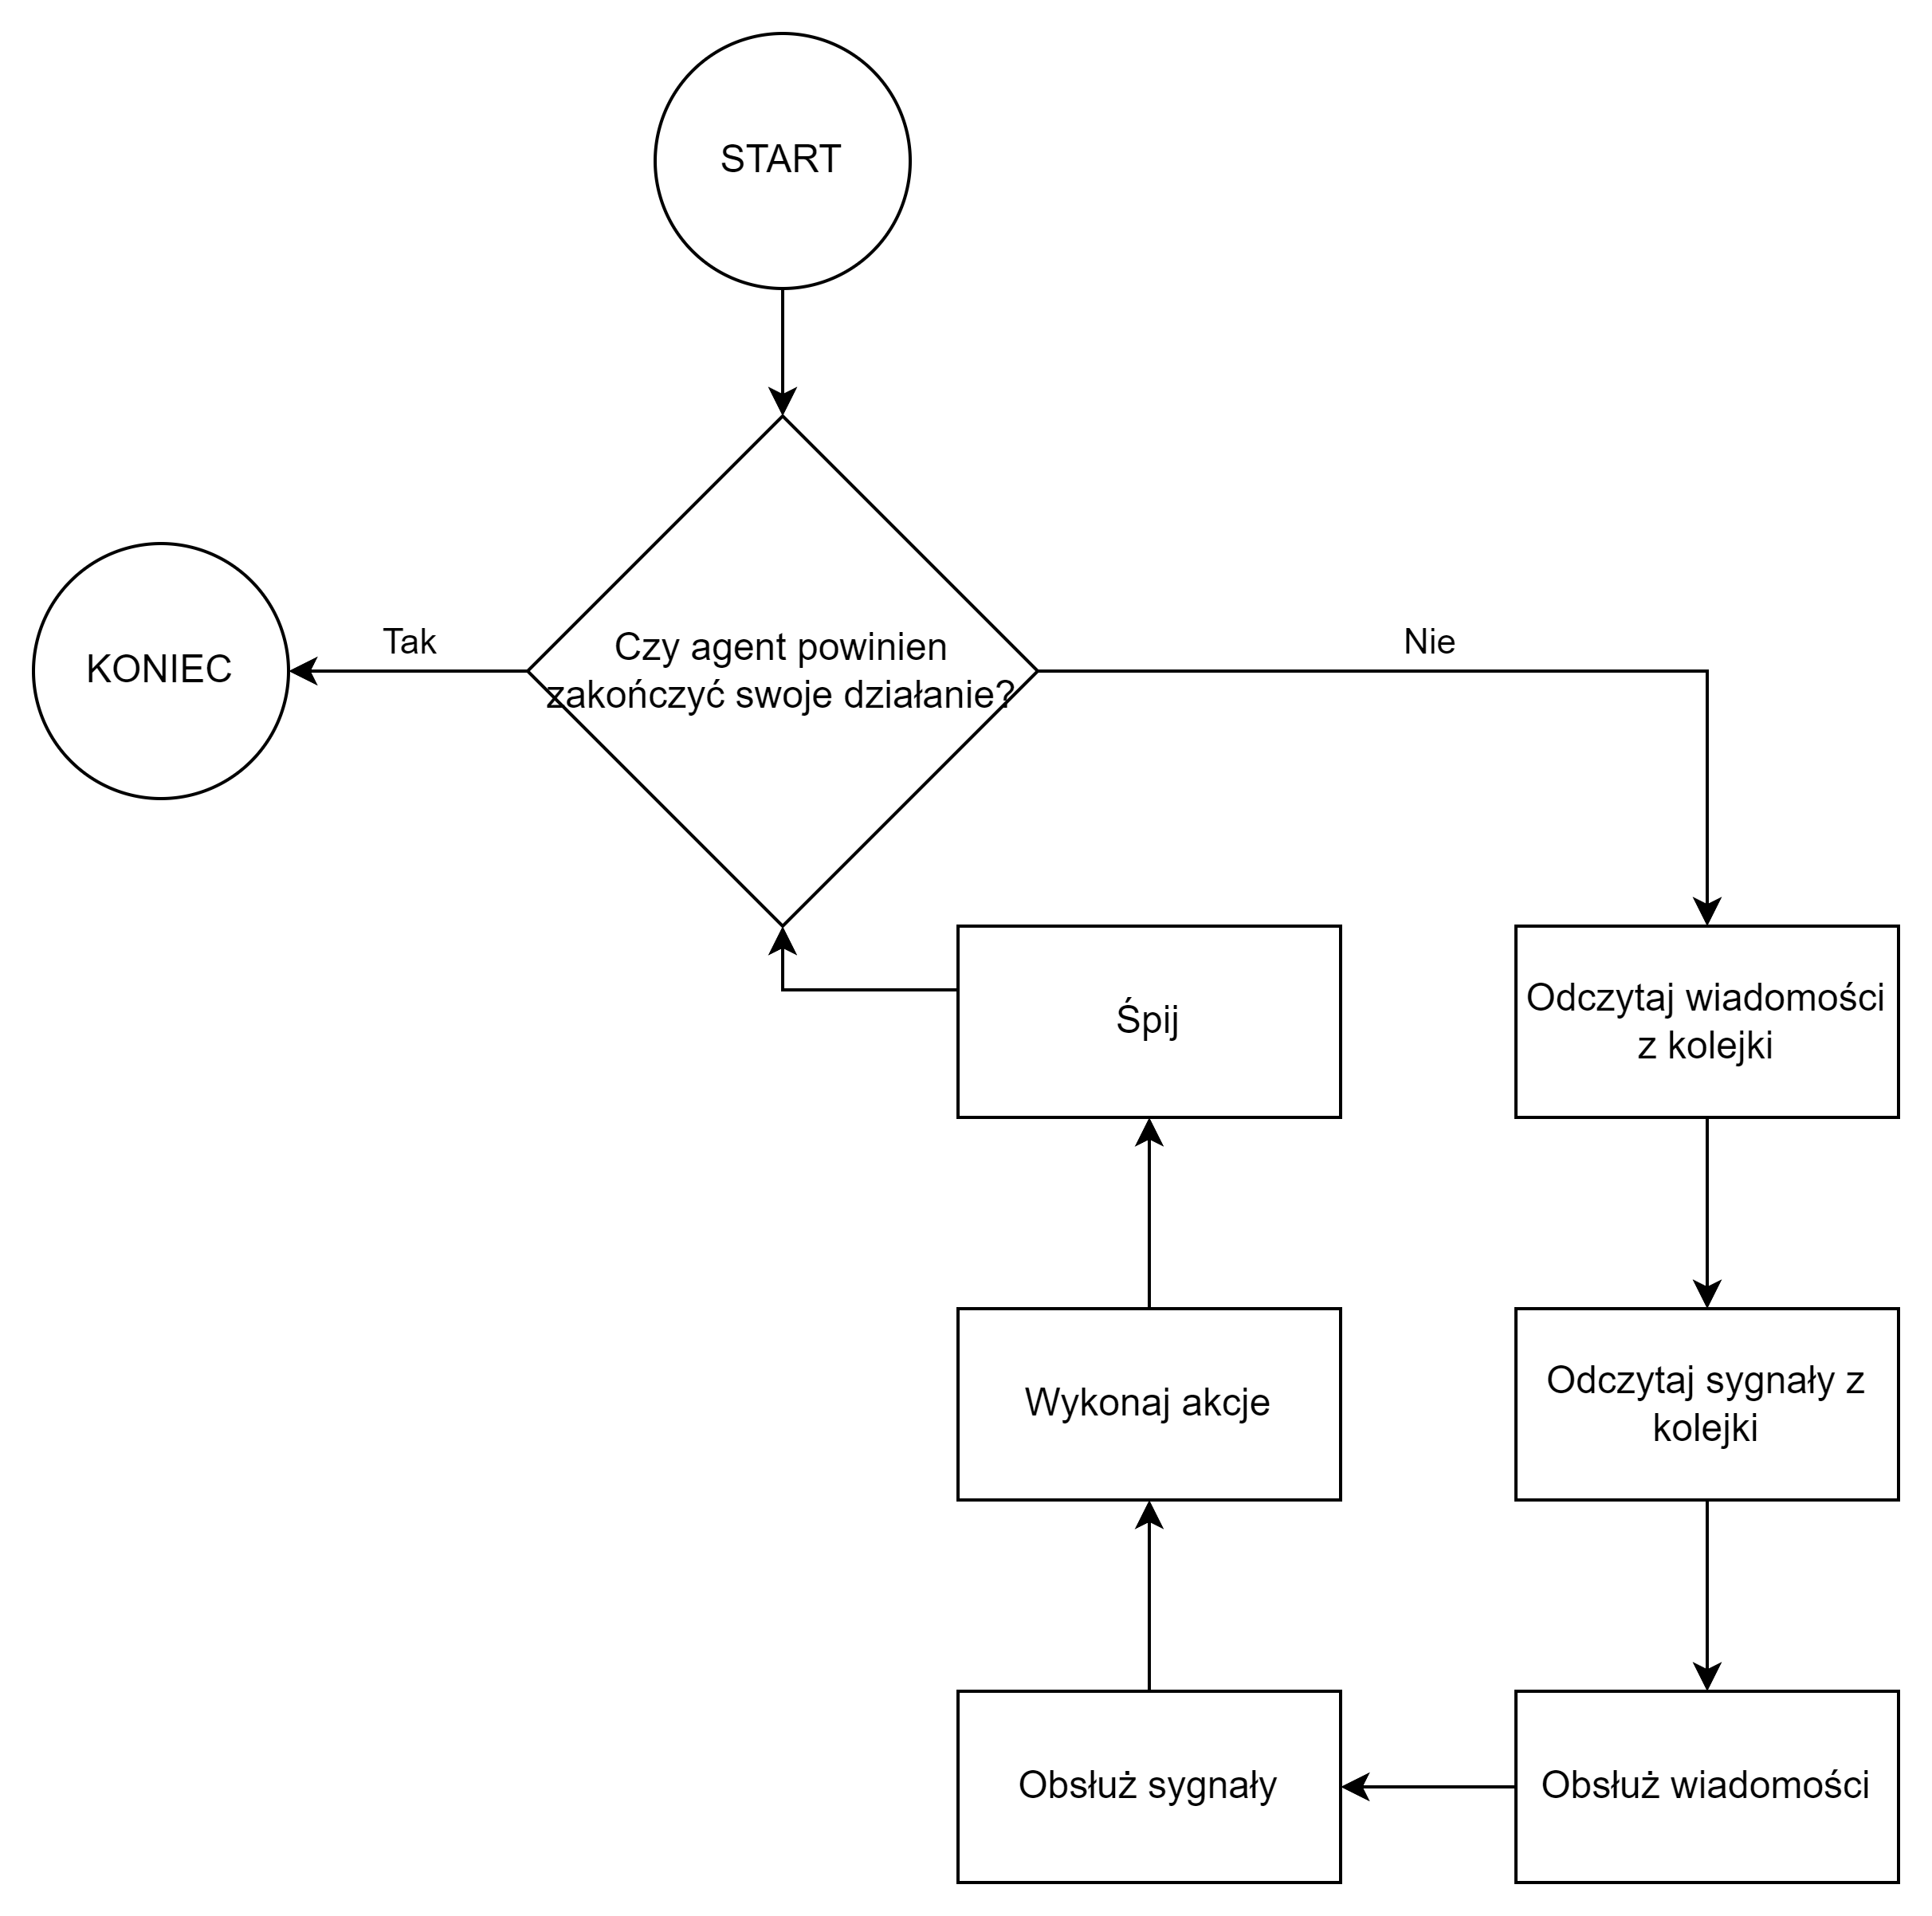
\includegraphics[width=\linewidth]{Agents - Agent Cycle}
    \caption{Cykl działania agenta}
    \label{fig:agentsAgentCycle}
    \source{Opracowanie Własne}
\end{figure}

\par Aby spełnić założenia systemu, ważnym było dokładne określenie wymiany wiadomości między agentami. Tabela \ref{tab:agentsMessagesSenderReceiver} pokazuje relację między typem wiadomości, a jej odbiorcą i nadawcą.

\begin{table}
    \centering
    \begin{tabular}{|c|c|c|} 
     \hline
     Rodzaj wiadomości & Nadawca & Odbiorca \\
     \hline
     \hline
     AskPositionMessage & Patrol Agent & Navigation Agent \\ 
     \hline
     CurrentLocationMessage & Navigation Agent & Patrol Agent \\ 
     \hline
     CurrentLocationMessage & Patrol Agent & HQ Agent \\ 
     \hline
     DestinationReachedMessage & Navigation Agent & Patrol Agent \\ 
     \hline
     GunFiredMessage & Gun Agent & Patrol Agent \\ 
     \hline
     GunFiredMessage & Patrol Agent & HQ Agent \\ 
     \hline
     IncidentInvestigationStartedMessage & Patrol Agent & HQ Agent \\ 
     \hline
     IncidentResolvedMessage & Patrol Agent & HQ Agent \\ 
     \hline
     JoinedShootingMessage & Patrol Agent & HQ Agent \\ 
     \hline
     NavigateToMessage & Patrol Agent & Navigation Agent \\ 
     \hline
     PatrolOfflineMessage & Patrol Agent & HQ Agent \\ 
     \hline
     PatrolOnlineMessage & Patrol Agent & HQ Agent \\ 
     \hline
     PatrolStatusChangedMessage & Patrol Agent & HQ Agent \\ 
     \hline
     ShowDistrictMessage & Patrol Agent & Navigation Agent \\ 
     \hline
     HandleIncidentOrderMessage & HQ Agent & Patrol Agent \\ 
     \hline
     PatrolDistrictOrderMessage & HQ Agent & Patrol Agent \\ 
     \hline
     SupportShootingOrderMessage & HQ Agent & Patrol Agent \\ 
     \hline
    \end{tabular}
    \caption{Tabela relacji wiadomości, nadawcy i odbiorcy}
    \label{tab:agentsMessagesSenderReceiver}
\end{table}

\par Zdefiniowane został również sygnały środowiskowe, służące agentom do obserwowania zmian w ich otoczeniu. Przedstawia je tabela \ref{tab:agentsEnvironmentSignals}.

\begin{table}
    \centering
    \begin{tabular}{|c|c|} 
     \hline
     Rodzaj sygnału & Agent \\
     \hline
     \hline
     DestinationReachedSignal & Navigation Agent \\ 
     \hline
     GunFiredSignal & Gun Agent \\ 
     \hline
     IncidentAlreadyOverSignal & Patrol Agent \\ 
     \hline
     IncidentResolvedSignal & Patrol Agent \\ 
     \hline
     PositionChangedSignal & Navigation Agent \\ 
     \hline
    \end{tabular}
    \caption{Tabela sygnałów środowiskowych wraz z ich odbiorcami}
    \label{tab:agentsEnvironmentSignals}
\end{table}

\par Aby komunikacja mogła nastąpić pomiędzy agentami, koniecznym jest ich odpowiednia konfiguracja. W szczególności dotyczy to patroli, które muszą wiedzieć, z jakich elementów się składają. W tym celu powstał interfejs \texttt{IPatrolInfoService}, który zapewnia informacje o identyfikatorach \emph{Patrol Agent}, \emph{Navigation Agent} i \emph{Gun Agent} oraz identyfikator patrolu, jako całości. Dokładniejszy opisz konfiguracji został omówiony w podrozdziale \ref{sec:konfiguracja}.